\documentclass{beamer}
\usetheme{dianahep}

%
% Title definitions
%

\title{Conceptualization of an NSF Scientific Software Innovation Institute for High Energy Physics (S2I2-HEP)}
\author{Peter Elmer - Princeton University \\
        Mark Neubauer - University of Illinois at Urbana-Champaign \\
        Mike Sokoloff - University of Cincinnati \\  
        \url{http://s2i2-hep.org}}
\date{1 May, 2018 \\ SI2 PI Meeting}

\begin{document}
\maketitle
%\insertframenumber/\inserttotalframenumber

%
% Presentation body
%

\setbeamertemplate{footline}[frame number]

% S2I2 HEP introdution

\begin{frame}
\frametitle{S2I2-HEP Conceptualization - http://s2i2-hep.org}

\begin{figure}[t]
\begin{center}
\includegraphics[width=0.9\textwidth]{images/s2i2-hep-website-banner.png}
%\caption{}
%\label{fig:example2}
\end{center}
\end{figure}

\small{The primary goal of the S2I2-HEP conceptualization project is to prepare a strategic plan for a potential NSF Scientific Software Innovation Institute (S2I2) to develop software for experiments taking data in the ``High-Luminosity Large Hadron Collider'' (HL-LHC) era in the 2020s.}
\vskip 0.1in
\small{S2I2-HEP sponsors community workshops and conceptual work to ``take advantage of the significant data and computing requirements of the Large Hadron Collider as a science driver for next generation high-performance software and sustainability developments.''}
\end{frame}



\begin{frame}
\frametitle{HEP Science Drivers - Beyond the ``Standard Model''}

The {\em Strategic Plan for U.S.\ Particle Physics} from May, 2014 (the
last community ``decadal survey'' and planning exercise for US HEP)
identified ``five compelling lines of inquiry that show 
great promise for discovery over the next 10 to 20 years.''
These are the Science Drivers:
\begin{itemize}
 \item Use the Higgs boson as a new tool for discovery
 \item Pursue the physics associated with neutrino mass
 \item Identify the new physics of dark matter
 \item Understand cosmic acceleration: dark matter and inflation
 \item Explore the unknown: new particles, interactions, and physical principles.
\end{itemize}

\end{frame}



\begin{frame}
\frametitle{Large Hadron Collider (LHC) and Experiments}

\begin{figure}[htbp]
\begin{center}
\includegraphics[width=0.8\textwidth]{images/CERNMap.jpg}
%\caption{}
%\label{fig:example2}
\end{center}
\end{figure}

\small{Two very large experiments (Atlas, CMS) with 3500+ people, and two large experiments (Alice, LHCb) with 500+ people}

\end{frame}



\begin{frame}
\frametitle{Worldwide LHC Computing Grid (WLCG)}

\begin{figure}[htbp]
\begin{center}
\includegraphics[width=0.9\textwidth]{images/WLCG-2017.png}
%\caption{}
%\label{fig:example2}
\end{center}
\end{figure}

\small{WLCG federates national grid infrastructures for the LHC experiments}

\end{frame}



\begin{frame}
\frametitle{Open Science Grid (OSG) - NSF}

\begin{figure}[htbp]
\begin{center}
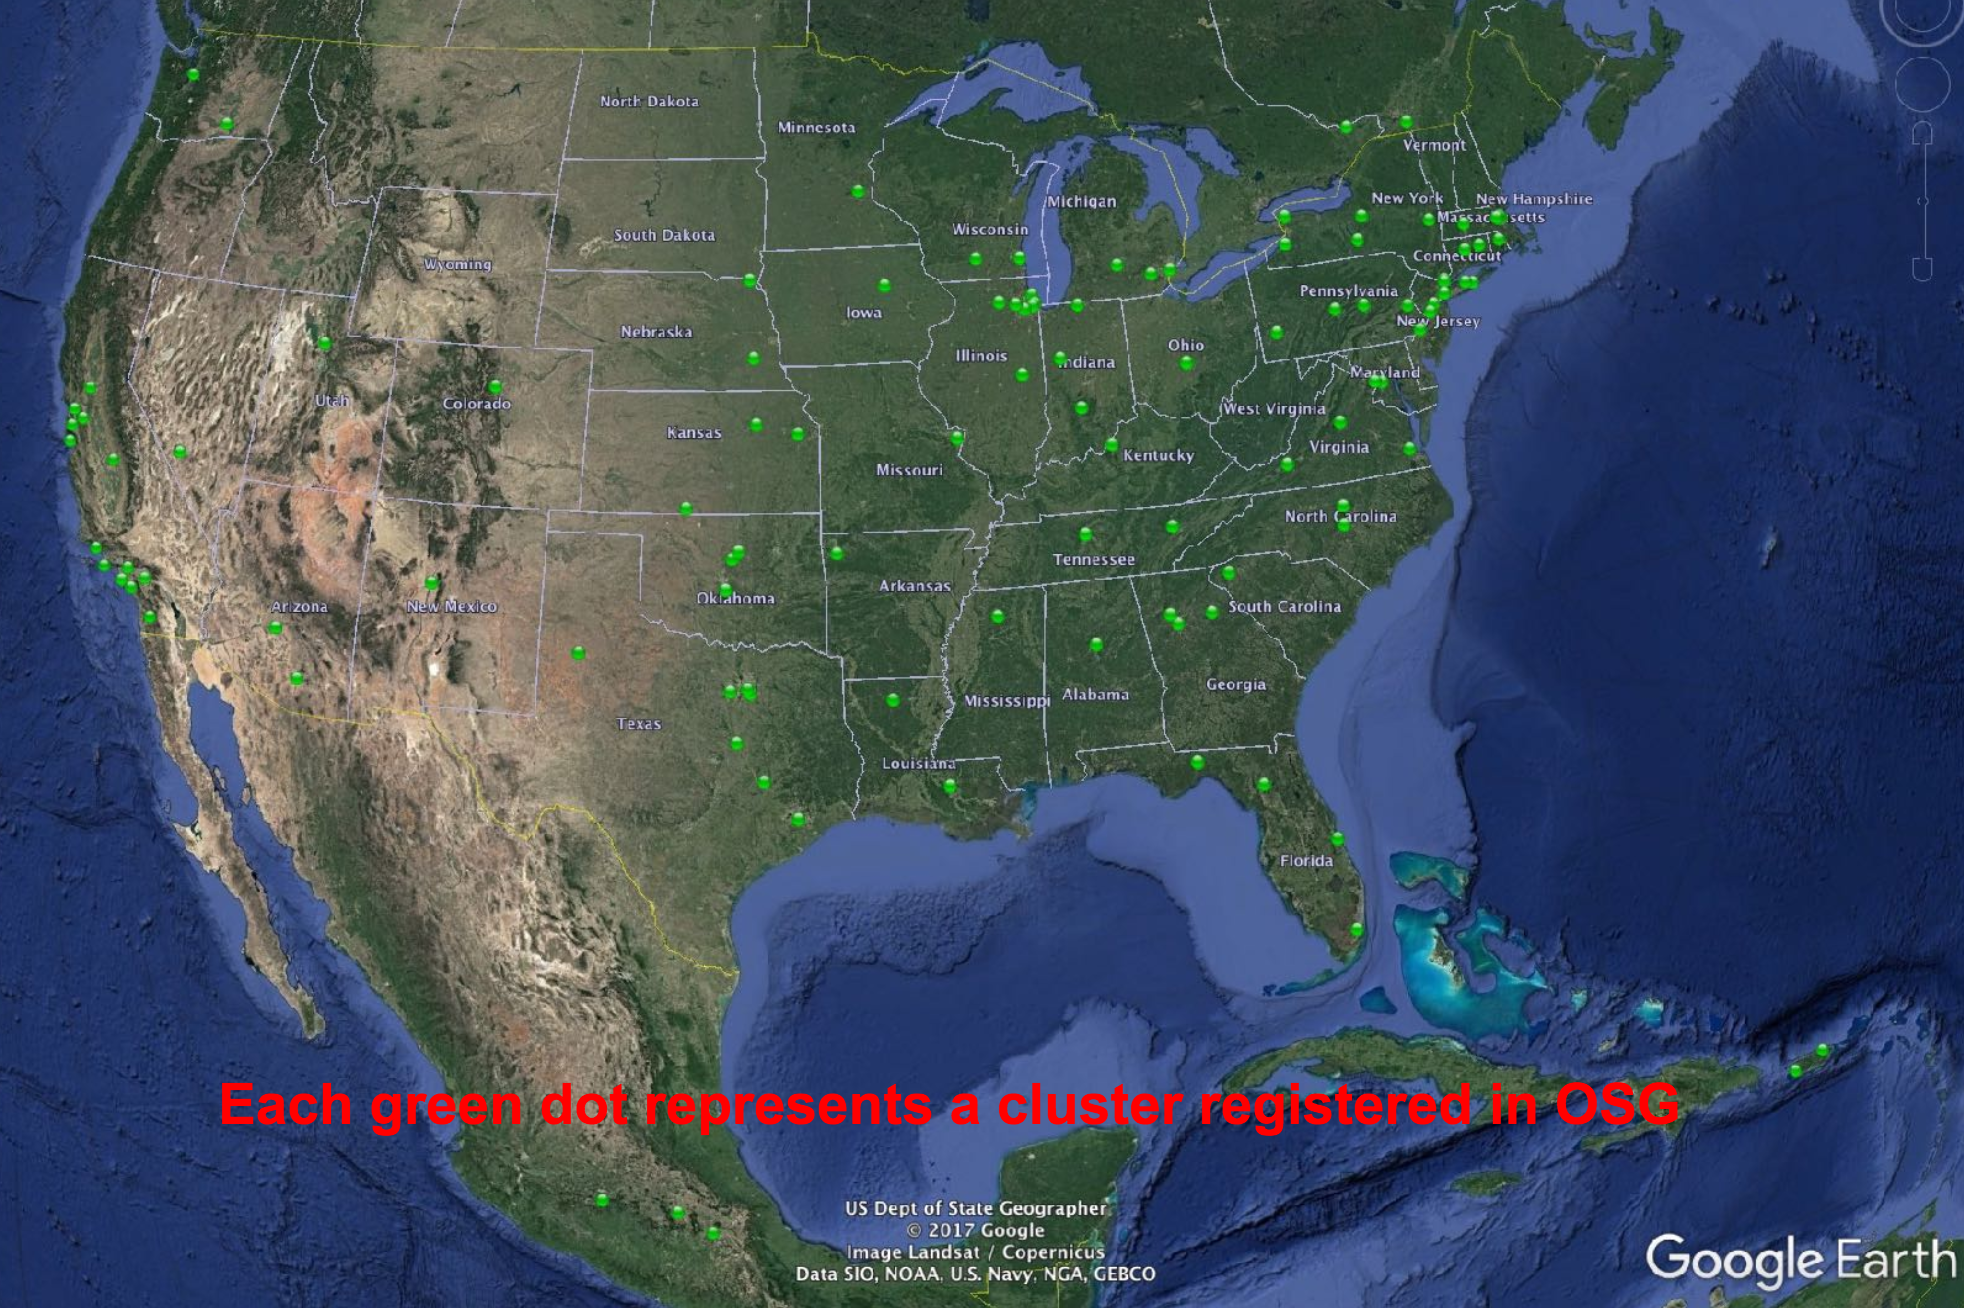
\includegraphics[width=0.8\textwidth]{images/osg-cluster-geography.png}
%\caption{}
%\label{fig:example2}
\end{center}
\end{figure}

\begin{center}
\small{In the US, OSG supports both LHC and many other sciences for DHTC}
\end{center}

\end{frame}



\begin{frame}
\frametitle{HEP Software Ecosystem}

\begin{figure}[htbp]
\begin{center}
\includegraphics[width=0.9\textwidth]{images/hep-software-ecosystem.jpg}
\end{center}
\end{figure}

{\small Plus 15-20M Source Lines of Code (SLOC) of ``experiment specific'' codes, as well as dependencies on non-HEP scientific software.}
\end{frame}



\begin{frame}
\frametitle{Plans for upgrading the LHC and Experiment Detectors}

\begin{figure}[htbp]
\begin{center}
\includegraphics[width=1.0\textwidth]{images/lhc-upgrade-timeline-detail.png}
%\caption{}
%\label{fig:example2}
\end{center}
\end{figure}

\small{The High Luminosity LHC Upgrade is a multi-national, multi-agency 
effort to realize the ultimate physics reach of the LHC. The NSF is
participating and preparations are underway
for a possible ``Major Research Equipment and Facilities Construction'' (MREFC) project to begin in $\sim$2020.}

\end{frame}



\begin{frame}
\frametitle{High Luminosity Challenges}

\begin{figure}[htbp]
\begin{center}
\includegraphics[width=1.0\textwidth]{images/hllhc-reco-tracking.png}
%\caption{}
%\label{fig:example2}
\end{center}
\end{figure}

%\small{Example Text}

\end{frame}



\input{slides/20180501-hllhc-compute-challenges-1.tex}
\begin{frame}
\frametitle{HL-LHC Computing Resources Estimate}

\begin{figure}[htbp]
\begin{center}
\includegraphics[width=0.8\textwidth]{images/hllhc-compute-challenges-brief-2.png}
%\caption{}
%\label{fig:example2}
\end{center}
\end{figure}

%\small{Example Text}

\end{frame}



\begin{frame}
\frametitle{August 2016 vision of Conceptualization Timeline}

\begin{figure}[htbp]
\begin{center}
\includegraphics[width=0.9\textwidth]{images/S2I2_timeline.png}
%\caption{}
%\label{fig:example2}
\end{center}
\end{figure}

%\small{Example Text}

\end{frame}



%\begin{frame}
\frametitle{Defining Longer-term Strategy}

\begin{itemize}
\item HL-LHC computing requires a major `software upgrade' and an eventual S2I2 institute for HEP would be a major player in that task
\item Planning for such an ``upgrade'' cannot be done for the US (Universities) in isolation
\item Thus we are intiating a larger community process to produce a Community White Paper (CWP) with an overall consensus strategy and roadmap for software and computing in HEP
  \begin{itemize}
  \item Initiated as WLCG charge to the LHC experiments and HSF as a step towards the LHC experiment TDRs in advance of HL-LHC
  \item The scope should not be restricted only to HL-LHC
  \item Some early software components could be built, tested and used by experiments in LHC Run3
  \end{itemize}
\item Organised by the HEP Software Foundation (HSF) [next slide]
\item Paper to be delivered by Summer 2017
\item The S2I2-HEP Strategic Plan will be derived from this global plan
\end{itemize}

\end{frame}



%\begin{frame}
\frametitle{CWP Charge}

[Switch to pdf file for CWP charge]

\end{frame}



\input{slides/20161207-hsf-intro-general.tex}
\begin{frame}
\frametitle{Community White Paper Process}

\begin{figure}[htbp]
\begin{center}
\includegraphics[width=0.95\textwidth]{images/hsf-cwp-timeline.png}
%\caption{}
%\label{fig:example2}
\end{center}
\end{figure}

%\small{Example Text}

\end{frame}



%\begin{frame}
\frametitle{(Switch to Webpages)}

S2I2-HEP (workshops) and papers: \url{http://s2i2-hep.org}
\vskip 0.15in
HSF CWP and WG: \url{http://hepsoftwarefoundation.org/activities/cwp.html}
\vskip 0.15in
HSF WG Start:
\url{http://hepsoftwarefoundation.org/cwp/cwp-wg-guidance-sdsc.html}
\end{frame}




\begin{frame}
\frametitle{Community White Paper}

\begin{figure}[htbp]
\begin{center}
\includegraphics[width=0.74\textwidth]{images/CWP-documents.png}
%\caption{}
%\label{fig:example2}
\end{center}
\end{figure}

%\small{Example Text}

\end{frame}




%\begin{frame}
\frametitle{Questions - Institute Focus Areas and Priorities}

{\scriptsize


\begin{enumerate}

\item {\bf Impact - Physics:} Will efforts in this area enable new approaches to computing and software that maximize, and could potentially radically extend, the physics reach of the detectors?
\item {\bf Impact - Resources:} Will efforts in this area achieve required improvements in software efficiency, scalability and performance and make use of the advances in CPU, storage and network technologies?
\item {\bf Impact - Sustainability:} Will efforts in this area guarantee the long term sustainability of the software through the lifetime of the HL-LHC?
\item {\bf Interest/Expertise:} Does the U.S.\ university community have a strong interest and expertise in the area?
\item {\bf Leadership:} Are the proposed focus areas complementary to efforts funded by the US-LHC Ops programs, DOE or international entities?
\item {\bf Value:} Is there potential to provide value to more than one LHC experiment and to the wider HEP community?
\item {\bf Research/Innovation:} Are there opportunities for combining research and innovation as part of partnerships between the HEP and Computer Science communities?
%\item Does the area offer opportunities for integration of cutting-edge training and education for our students and postdocs?
\end{enumerate}




}

\end{frame}



\begin{frame}
\frametitle{S2I2-HEP Impact Criteria (for evaluating each WG topic)}

\begin{enumerate}
\item {\bf Impact - Physics:} Will efforts in this area enable new approaches to computing and software that maximize, and could potentially radically extend, the physics reach of the detectors?
\item {\bf Impact - Resources:} Will efforts in this area achieve required improvements in software efficiency, scalability and performance and make use of the advances in CPU, storage and network technologies?
\item {\bf Impact - Sustainability:} Will efforts in this area guarantee the long term sustainability of the software through the lifetime of the HL-LHC?
\end{enumerate}
\end{frame}



\begin{frame}
\frametitle{Additional Criteria (for prioritization)}

\begin{enumerate}
\item {\bf Interest/Expertise:} Does the U.S.\ university community have a strong interest and expertise in the area?
\item {\bf Leadership:} Are the proposed focus areas complementary to efforts funded by the US-LHC Ops programs, DOE or international entities?
\item {\bf Value:} Is there potential to provide value to more than one LHC experiment and to the wider HEP community?
\item {\bf Research/Innovation:} Are there opportunities for combining research and innovation as part of partnerships between the HEP and Computer Science communities?
\end{enumerate}

\end{frame}



\begin{frame}
\frametitle{Strategic Plan - 4 Priority R\&D Focus Areas}

\vskip 0.15in
\noindent{\bf Analysis Systems:} Maximize scientific potential; high-throughput, low-latency systems minimizing ``time-to-insight''; reuse and reproducibility integrated
\vskip 0.15in
\noindent{\bf Data Organization, Management and Access (DOMA):} tools to meet the challenges of organizing, managing, and providing access to exabytes of data from processing systems of various kinds.
\vskip 0.15in
\noindent{\bf Reconstruction/Trigger (Algorithms):} Computationally intensive algorithms and implementations for real-time data selection, pattern recognition, etc.
\vskip 0.15in
\noindent{\bf Applications of Machine Learning:} Leverage wider advances in ML and Data Science

\end{frame}



\input{slides/20180501-s2i2-hep-institute-structure.tex}
\begin{frame}
\frametitle{Blueprint Process}

\begin{figure}[htbp]
\begin{center}
\includegraphics[width=0.8\textwidth]{images/s2i2-global-blueprint-activity.png}
%\caption{}
%\label{fig:example2}
\end{center}
\end{figure}

\small{The Blueprint Process will be a primary means of developing a common vision with the major partners. Blueprint activities will likely happen 3-4 times per year, typically with a focus on a different specific topics each time.}

\end{frame}



\begin{frame}
\frametitle{Continuing Integration - WLCG/HSF Workshop}

\begin{figure}[htbp]
\begin{center}
\includegraphics[width=0.8\textwidth]{images/small-naples-group-photo.JPG}
%\caption{}
%\label{fig:example2}
\end{center}
\end{figure}

\begin{center}
\small{Worldwide LHC Computing Grid/HEP Software Foundation - Mar 2018}
\end{center}

\end{frame}



\begin{frame}
\frametitle{Summary}

\begin{itemize}
\item Significant challenges and scientific opportunities for the HEP community at the High Luminosity LHC in the 2020s: realize the full physics potential of a decades long international investment.
\item The S2I2-HEP conceptualization project drove both an international
and a US national planning during 2017
\item Major deliverables:
   \begin{itemize}
   \item Community White Paper: A Roadmap for HEP Software and Computing R\&D for the 2020s
   \item Strategic Plan for a Scientific Software Innovation Institute (S2I2) for High Energy Physics
   \item Significantly increased HEP community integration and collaboration
   \end{itemize}
\end{itemize}

\end{frame}




\end{document}


